%-------------------------------------------------------------------------
% Design Project Input/Output Module Description
%-------------------------------------------------------------------------

\clearpage
\section{Piezo Output Module}
\label{sec-output-piezo}

This output module enables your IoT device to play tones using a piezo
element. A piezo element makes a clicking sound each time it is pulsed
with current. If we pulse it at the right frequency (for example 440
times a second to make the note middle A), these clicks produce notes.

A sample circuit and Arduino code is shown below to get you started.
Note that the piezo element is powered directly from the Arduino signal
pin. There is no need for any extra components; with the rectangular
"TDX" label facing to your left, we directly connect the left lead of
the piezo element to a digital output PWM pin on the Arduino and the
right lead to ground.

The example code has two experiments. In the first, we play a middle A
by pulsing the piezo element with a square wave at \wu{440}{Hz} -- i.e.,
\wu{1136}{\textmu{}s} HIGH and \wu{1136}{\textmu{}s} LOW. In the second
experiment, we play a tune using the playNote() library function. You
can use this function by giving it a note name (see the table below for
notes) and a duration to play the note; the function will play the note
using the same technique we saw in the first experiment. After setting
up the circuit and programming the Arduino, listen to the notes produced
by the piezo element and see if it makes sense. You can then experiment
with other tunes by choosing your own notes! The table below lists the
frequencies, periods, and the time to pulse the piezo element to play
different notes across two octaves.

%FIXME: The code needs to be modified to choose between experiments 1 and 2.

\vspace{0.1in}
\begin{minipage}[t]{0.49\tw}
  \vspace{0.0in}
  \centering
    \begin{tabular}{c|c|c|c}
    \BF{Note Name} & \BF{Frequency} & \BF{Period} & \BF{Time High}\\\hline
    C              & \wu{131}{Hz}   & 7634        & 3817 \\
    D              & \wu{147}{Hz}   & 6802        & 3401 \\
    E              & \wu{165}{Hz}   & 6060        & 3030 \\
    F              & \wu{175}{Hz}   & 5714        & 2857 \\
    G              & \wu{196}{Hz}   & 5102        & 2551 \\
    A              & \wu{220}{Hz}   & 4546        & 2273 \\
    B              & \wu{247}{Hz}   & 4048        & 2024 \\
    c              & \wu{261}{Hz}   & 3830        & 1915 \\
    d              & \wu{294}{Hz}   & 3400        & 1700 \\
    e              & \wu{329}{Hz}   & 3038        & 1519 \\
    f              & \wu{349}{Hz}   & 2864        & 1432 \\
    g              & \wu{392}{Hz}   & 2550        & 1275 \\
    a              & \wu{440}{Hz}   & 2272        & 1136 \\
    b              & \wu{493}{Hz}   & 2028        & 1014 \\
    \end{tabular}
  \centering

  \vspace{0.15in}
  \begin{Verbatim}[gobble=3,fontsize=\small]
    // Experiment 1: Playing a note

    #include <Piezo.h>

    int pin_piezo = 6;

    void setup() {
      pinMode( pin_piezo, OUTPUT );
    }

    void loop() {

      // Play an A4 ( 440Hz, 2272us period ).
      // Dividing the period by 2 makes 1136us --
      // the time we hold the signal HIGH or LOW.

      while (1) {
        digitalWrite( pin_piezo, HIGH );
        delayMicroseconds( 1136 );
        digitalWrite( pin_piezo, LOW );
        delayMicroseconds( 1136 );
      }
    }
  \end{Verbatim}

\end{minipage}
\hspace{0.1in}
\begin{minipage}[t]{0.49\tw}
  \vspace{0.0in}
  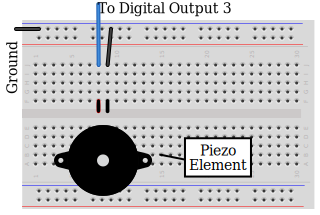
\includegraphics[width=\tw]{output-piezo-annotated.svg.pdf}

  \vspace{0.7in}
  \begin{Verbatim}[gobble=3,fontsize=\small]
    // Experiment 2: Playing a tune

    #include <Piezo.h>

    int pin_piezo = 6;

    void setup() {
      pinMode( pin_piezo, OUTPUT );
    }

    void loop() {

      // Set up the tune. The length is the
      // number of notes. The notes array
      // contains the tune -- a space is a
      // rest. The beats array contains how
      // many beats each note should take.

      int length   = 30;
      char notes[] = "ABcGGdcBAAAABcABcGGdcdeefedcdc ";
      int beats[]  = { 1, 1, 6, 1, 1, 6, 1, 1,
                       1, 1, 2, 1, 2, 6,
                       1, 1, 6, 1, 1, 6, 1, 1,
                       1, 2, 2, 1, 1, 1, 1, 4, 4 };
      int tempo    = 100;

      // Play tune using the playNote() function.

      for (int i = 0; i < length; i++) {
        playNote(pin_piezo, notes[i], beats[i] * tempo);
        delay(tempo / 2); // Pause between notes
      }

    }
  \end{Verbatim}
\end{minipage}
\vspace{0.1in}

%Questions:
